\documentclass[12pt, a4paper]{book}

\usepackage[T1]{fontenc}
\usepackage[utf8]{inputenc}
\usepackage[charter, cal=cmcal]{mathdesign}
\usepackage[scaled=0.92]{helvet}
\usepackage{geometry}
\geometry{a4paper, top=30mm, bottom=30mm, inner=32mm, outer=25mm, marginparwidth=18mm}

\usepackage{amsmath, amsthm}
\usepackage[version=4]{mhchem}
\usepackage{graphicx}
\usepackage{xcolor}
\usepackage{tikz}
\usetikzlibrary{arrows.meta, shapes.geometric, positioning, calc, backgrounds}
\usepackage{pgfplots}
\pgfplotsset{compat=1.18}
\usepackage{tcolorbox}
\tcbuselibrary{skins, breakable, theorems}
\usepackage{titlesec}
\usepackage{fancyhdr}
\usepackage{enumitem}
\usepackage{booktabs}
\usepackage{array}
\usepackage{parskip}
\usepackage{siunitx}
\usepackage[colorlinks=true, linkcolor=BrickRed,
            urlcolor=NavyBlue, citecolor=ForestGreen]{hyperref}

% ── Colours (Journey 8 — forest green / amber) ────────────────────────────────
\definecolor{JourneyColor}{HTML}{065F46}
\definecolor{ModuleColor}{HTML}{059669}
\definecolor{PuzzleColor}{HTML}{B45309}
\definecolor{DiscoveryColor}{HTML}{D97706}
\definecolor{WarningColor}{HTML}{991B1B}
\definecolor{ProblemColor}{HTML}{6B21A8}
\definecolor{ReflectColor}{HTML}{0D9488}
\definecolor{HistoryColor}{HTML}{78350F}

% ── Boxes ─────────────────────────────────────────────────────────────────────
\newtcolorbox{puzzlebox}[1][]{enhanced,breakable,
  colback=PuzzleColor!6,colframe=PuzzleColor,fonttitle=\bfseries\sffamily,
  title={The Puzzle},attach boxed title to top left={yshift=-2mm,xshift=6mm},
  boxed title style={colback=PuzzleColor},borderline west={3pt}{0pt}{PuzzleColor},#1}

\newtcolorbox{discoverybox}[1][]{enhanced,breakable,
  colback=DiscoveryColor!8,colframe=DiscoveryColor,fonttitle=\bfseries\sffamily,
  title={Discovery},attach boxed title to top left={yshift=-2mm,xshift=6mm},
  boxed title style={colback=DiscoveryColor},borderline west={3pt}{0pt}{DiscoveryColor},#1}

\newtcolorbox{problembox}[1][]{enhanced,breakable,
  colback=ProblemColor!5,colframe=ProblemColor,fonttitle=\bfseries\sffamily,
  title={Problems},attach boxed title to top left={yshift=-2mm,xshift=6mm},
  boxed title style={colback=ProblemColor},borderline west={3pt}{0pt}{ProblemColor},#1}

\newtcolorbox{deepbox}[1][]{enhanced,breakable,
  colback=JourneyColor!5,colframe=JourneyColor,fonttitle=\bfseries\sffamily,
  title={Deep Problems},attach boxed title to top left={yshift=-2mm,xshift=6mm},
  boxed title style={colback=JourneyColor},borderline west={4pt}{0pt}{JourneyColor},#1}

\newtcolorbox{historybox}[1][]{enhanced,breakable,
  colback=HistoryColor!7,colframe=HistoryColor!60,fonttitle=\bfseries\sffamily\small,
  title={Historical Note},attach boxed title to top left={yshift=-2mm,xshift=6mm},
  boxed title style={colback=HistoryColor!80},#1}

\newtcolorbox{reflectionbox}[1][]{enhanced,breakable,
  colback=ReflectColor!6,colframe=ReflectColor,fonttitle=\bfseries\sffamily,
  title={Reflection},attach boxed title to top left={yshift=-2mm,xshift=6mm},
  boxed title style={colback=ReflectColor},borderline west={3pt}{0pt}{ReflectColor},#1}

\newtcolorbox{namedconcept}[2][]{enhanced,
  colback=ModuleColor!6,colframe=ModuleColor,fonttitle=\bfseries\sffamily\large,
  title={#2},attach boxed title to top left={yshift=-2mm,xshift=6mm},
  boxed title style={colback=ModuleColor},#1}

% ── Section formatting ────────────────────────────────────────────────────────
\titleformat{\chapter}[display]
  {\normalfont\sffamily\huge\bfseries\color{JourneyColor}}
  {\textcolor{JourneyColor!60}{\chaptertitlename\ \thechapter}}{10pt}{\Huge}
  [\vspace{2pt}\textcolor{JourneyColor}{\titlerule[1.5pt]}]
\titleformat{\section}
  {\normalfont\sffamily\Large\bfseries\color{ModuleColor}}
  {\thesection}{1em}{}[\textcolor{ModuleColor!40}{\titlerule[0.6pt]}]
\titleformat{\subsection}
  {\normalfont\sffamily\large\bfseries\color{JourneyColor!80}}{\thesubsection}{1em}{}
\titleformat{\subsubsection}
  {\normalfont\sffamily\normalsize\bfseries}{\thesubsubsection}{1em}{}

\pagestyle{fancy}
\fancyhf{}
\fancyhead[LE]{\small\sffamily\textcolor{JourneyColor}{\leftmark}}
\fancyhead[RO]{\small\sffamily\textcolor{ModuleColor}{\rightmark}}
\fancyfoot[C]{\small\thepage}
\renewcommand{\headrulewidth}{0.4pt}

\newcommand{\newterm}[1]{\textit{\textcolor{DiscoveryColor}{#1}}}
\newcommand{\important}[1]{\textcolor{ModuleColor}{\textbf{#1}}}

\begin{document}

\setcounter{chapter}{7}
\setcounter{section}{3}

\section{Module 8.4 --- Ceramics, Glasses, and Nanomaterials}

At the boundaries of solid-state structure lie materials that challenge simple definitions of crystal order. Ceramics utilize strong ionic and covalent bonding networks to achieve high thermal and chemical stability, but remain brittle. Glasses bypass crystallization entirely, forming amorphous solids. Finally, as the dimensions of a material shrink to the nanometer scale, bulk properties collapse, and quantum mechanics dictates a size-dependent color and reactivity.

\newpage

% ─── Section: The Puzzle ─────────────────────────────────────────────────────
\section{Part 1 --- The Puzzle}

\begin{puzzlebox}
\textbf{The Surface-to-Volume Explosion}

Suppose we have a single spherical gold particle of radius $R = \SI{1}{cm}$. We slice this gold sphere repeatedly to produce tiny nanocrystals of radius $r = \SI{2}{nm}$.

\medskip
\begin{center}
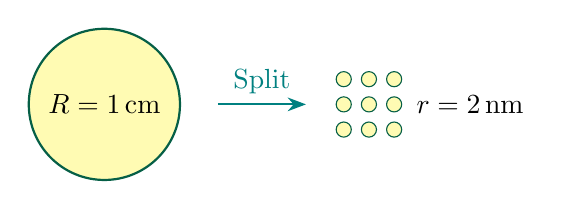
\begin{tikzpicture}[scale=0.8]
  % Draw a large sphere representation
  \draw[fill=yellow!30, draw=JourneyColor, thick] (0,0) circle (1.2);
  \node at (0,0) {$R = \SI{1}{cm}$};
  
  \draw[->, >=Stealth, thick, teal] (1.8,0) -- (3.2,0) node[midway, above] {Split};
  
  % Draw many tiny spheres representation
  \foreach \x in {3.8,4.2,4.6} {
    \foreach \y in {-0.4,0,0.4} {
      \draw[fill=yellow!30, draw=JourneyColor] (\x,\y) circle (0.12);
    }
  }
  \node[right] at (4.8, 0) {$r = \SI{2}{nm}$};
\end{tikzpicture}
\end{center}

\medskip
\textbf{Question 1.} Calculate the ratio of the total surface area of all the tiny spheres to the surface area of the original large sphere. If each gold atom occupies a volume of $\approx \SI{1.7e-23}{cm^3}$ and has a radius of $\approx \SI{0.144}{nm}$, what fraction of the total gold atoms reside on the surface in the nanocrystals compared to the bulk sphere?

\textbf{Question 2.} Atoms at the surface of a material have fewer neighbors than those in the bulk. What does this imply for the chemical reactivity and thermodynamic stability of surface atoms?

\textbf{Question 3.} Bulk gold is highly inert and has a shiny yellow color. Gold nanoparticles, however, appear ruby red or purple in solution and act as powerful catalysts. Why does a simple change in physical dimension alter both optical and chemical properties?
\end{puzzlebox}

\newpage

% ─── Section: Exploration ────────────────────────────────────────────────────
\section{Part 2 --- Exploration}

\subsection{Step 1: The Glass Transition and Amorphous Structures}

\begin{problembox}
When a liquid is cooled, it typically crystallizes at its melting temperature $T_m$, resulting in a discontinuous drop in volume and entropy. If the cooling rate is extremely rapid, the liquid can be supercooled below $T_m$ without crystallizing. At a lower temperature $T_g$, the viscosity increases so dramatically ($\eta > \SI{10^{12}}{Pa\cdot s}$) that the atoms are locked into an amorphous, non-crystalline arrangement. This is the **glass transition**.

\begin{enumerate}[label=(\alph*)]
  \item Draw a schematic plot of volume (or enthalpy) versus temperature for a material cooled slowly (crystallization) and cooled rapidly (glass formation). Highlight the melting temperature $T_m$ and the glass transition temperature $T_g$.
  \item Silica ($\ce{SiO2}$) forms both crystalline quartz and amorphous silica glass. In quartz, $\ce{SiO4}$ tetrahedra are arranged in a periodic 3D network. In silica glass, they share corners but lack long-range periodic order. Explain why silica glass is mechanically isotropic (has the same properties in all directions), whereas quartz is anisotropic.
  \item Why does adding network modifiers like sodium oxide ($\ce{Na2O}$) or calcium oxide ($\ce{CaO}$) to silica lower its melting and glass transition temperatures? (Consider the effect of these modifiers on the connectivity of the covalent network).
\end{enumerate}
\end{problembox}

\subsection{Step 2: Quantum Confinement and the Brus Equation}

\begin{problembox}
In a semiconductor nanocrystal (a **quantum dot**), the size of the crystal is smaller than the exciton Bohr radius (the natural separation distance of a photo-excited electron-hole pair). Under these conditions, the carriers are quantum-mechanically confined in 3D. We model the exciton as a particle in a 3D spherical box of radius $R$.

The band gap of the quantum dot $E_{g,\text{QD}}$ is shifted relative to the bulk band gap $E_{g,\text{bulk}}$ according to the **Brus Equation**:
\[
  E_{g,\text{QD}} \;=\; E_{g,\text{bulk}} + \frac{h^2}{8 R^2}\left(\frac{1}{m_e^*} + \frac{1}{m_h^*}\right) - \frac{1.8 q^2}{4\pi \varepsilon R},
\]
where $m_e^*$ is the effective mass of the electron, $m_h^*$ is the effective mass of the hole, and the third term represents the Coulombic attraction between the electron and the hole.

\begin{enumerate}[label=(\alph*)]
  \item Show that as the radius $R$ of the quantum dot decreases, the band gap energy increases. Which term in the Brus equation dominates at very small dimensions?
  \item Explain why cadmium selenide (CdSe) quantum dots emit blue light when they are small ($R \approx \SI{1.5}{nm}$) and red light when they are larger ($R \approx \SI{4}{nm}$).
  \item Why is this size-dependent color control impossible in bulk CdSe?
\end{enumerate}
\end{problembox}

\newpage

% ─── Section: Discovery ──────────────────────────────────────────────────────
\section{Part 3 --- Discovery}

\begin{discoverybox}
\textbf{The Thermodynamics of Surfaces and Nucleation}

Every surface carries a thermodynamic cost. The work required to create an interface of area $A$ is given by $W = \gamma A$, where $\gamma$ is the \newterm{surface energy}. This term dominates when materials are synthesized or when a phase transition begins.

In the nucleation of a solid phase from a supercooled liquid, the change in Gibbs free energy to form a spherical solid nucleus of radius $r$ is:
\[
  \Delta G(r) \;=\; -\frac{4}{3}\pi r^3 \Delta G_v + 4\pi r^2 \gamma,
\]
where $\Delta G_v$ is the chemical driving force per unit volume (favorable for crystallization) and $\gamma$ is the solid-liquid surface energy (unfavorable).

\begin{center}
\begin{tikzpicture}[scale=0.8]
  \begin{axis}[
    axis lines=middle,
    xmin=0, xmax=3,
    ymin=-5, ymax=5,
    ticks=none,
    xlabel={$r$},
    ylabel={$\Delta G$},
    every axis x label/.style={at={(current axis.right of origin)},anchor=west},
    every axis y label/.style={at={(current axis.above origin)},anchor=south}
  ]
    \addplot[domain=0:2.5, samples=100, thick, JourneyColor] {-4*x^3 + 6*x^2};
    \draw[dashed, darkgray] (1.0, -10) -- (1.0, 2.0) node[above] {$r^*$};
  \end{axis}
\end{tikzpicture}
\end{center}

Differentiating $\Delta G$ with respect to $r$ yields the **critical nucleation radius** $r^* = \frac{2\gamma}{\Delta G_v}$. Nuclei with $r < r^*$ are unstable and shrink to lower their energy, while nuclei with $r > r^*$ are stable and grow spontaneously.
\end{discoverybox}

\newpage

% ─── Section: What This Is Called ────────────────────────────────────────────
\section{Part 4 --- What This Is Called}

\begin{namedconcept}{Amorphous and Nanoscale Physics}
\begin{itemize}
  \item \important{Network Former:} A covalent oxide that forms a continuous 3D network of bonded polyhedra (e.g., $\ce{SiO2}$, $\ce{B2O3}$).
  \item \important{Network Modifier:} Ionic oxides added to glass that break the covalent bonds of the network, converting bridging oxygens into non-bridging oxygens (e.g., $\ce{Na2O}$).
  \item \important{Quantum Confinement:} The restriction of charge carriers in dimensions comparable to or smaller than their de Broglie wavelength.
  \item \important{Exciton:} A bound state of an electron and an electron hole held together by the Coulomb force.
\end{itemize}
\end{namedconcept}

\newpage

% ─── Section: Solved Exercises ───────────────────────────────────────────────
\section{Part 5 --- Solved Exercises}

\begin{problembox}
\textbf{Exercise:} Calculate the critical nucleation radius $r^*$ and the activation energy barrier $\Delta G^*$ for the solidification of copper, given:
* Melting temperature $T_m = \SI{1356}{K}$.
* Under cooling $\Delta T = T_m - T = \SI{200}{K}$.
* Latent heat of fusion $\Delta H_f = \SI{1.63e9}{J/m^3}$.
* Surface energy $\gamma = \SI{0.177}{J/m^2}$.
Use the approximation $\Delta G_v \approx \frac{\Delta H_f \Delta T}{T_m}$.

\textbf{Solution:}
\begin{enumerate}
  \item First, calculate the volume free energy change $\Delta G_v$:
        \[
          \Delta G_v \;=\; \frac{1.63e9 \times 200}{1356} \;\approx\; \SI{2.404e8}{J/m^3}.
        \]
  \item Find the critical radius $r^*$:
        \[
          r^* \;=\; \frac{2\gamma}{\Delta G_v} \;=\; \frac{2 \times 0.177}{2.404e8} \;\approx\; \SI{1.47e-9}{m} \;=\; \SI{1.47}{nm}.
        \]
  \item The activation energy barrier $\Delta G^*$ occurs at $r = r^*$:
        \[
          \Delta G^* \;=\; \Delta G(r^*) \;=\; \frac{16\pi \gamma^3}{3 (\Delta G_v)^2}.
        \]
        Substitute the values:
        \[
          \Delta G^* \;=\; \frac{16\pi \times (0.177)^3}{3 \times (2.404e8)^2} \;\approx\; \frac{0.2787}{1.734e17} \;\approx\; \SI{1.61e-18}{J}.
        \]
        Dividing by $k_B T \approx 1.38e-23 \times 1156 \approx \SI{1.60e-20}{J}$, we find $\Delta G^* / k_B T \approx 100$. This high barrier means homogeneous nucleation is extremely slow, and solidification must rely on foreign particles (heterogeneous nucleation).
\end{enumerate}
\end{problembox}

\newpage

% ─── Section: Problems ───────────────────────────────────────────────────────
\section{Part 6 --- Problems}

\begin{problembox}
\begin{enumerate}[label=\textbf{P\arabic*.}]
  \item \textbf{Silicate Glass Network Topology.}
  
        Silicate glasses are characterized by the ratio of oxygen to silicon atoms ($O/Si$).
        \begin{enumerate}[label=(\alph*)]
          \item In pure silica ($\ce{SiO2}$), $O/Si = 2$. What fraction of oxygen atoms share two silicon atoms (bridging oxygens)?
          \item We add sodium oxide to create a glass with composition $\ce{Na2Si2O5}$. Calculate the $O/Si$ ratio.
          \item Show that for $\ce{Na2Si2O5}$, on average one oxygen per silicon tetrahedron is non-bridging. How does this modify the structural rigidity of the glass?
        \end{enumerate}

  \item \textbf{The Surface Melting Depress.}
  
        Because surface atoms have fewer bonds, they melt at a lower temperature than bulk atoms. The melting point $T_m(D)$ of a nanoparticle of diameter $D$ can be modeled as:
        \[
          T_m(D) \;=\; T_{m,\text{bulk}} \left(1 - \frac{4\sigma_{sl}}{\rho_s H_f D}\right),
        \]
        where $\sigma_{sl} \approx \SI{0.12}{J/m^2}$ is the solid-liquid surface tension, $\rho_s \approx \SI{1.93e4}{kg/m^3}$ is the density of gold, and $H_f \approx \SI{6.3e4}{J/kg}$ is the latent heat of fusion.
        \begin{enumerate}[label=(\alph*)]
          \item Calculate the melting temperature of a gold nanoparticle with $D = \SI{3}{nm}$, given $T_{m,\text{bulk}} = \SI{1337}{K}$.
          \item Discuss the implications of this size-dependent melting for the stability of nanoscale electronic interconnects.
        \end{enumerate}
\end{enumerate}
\end{problembox}

\newpage

% ─── Section: Deep Problems ──────────────────────────────────────────────────
\section{Part 7 --- Deep Problems}

\begin{deepbox}
\begin{enumerate}[label=\textbf{D\arabic*.}]
  \item \textbf{The Brus Equation Coulomb Term Derivation.}
  
        The Brus equation contains a kinetic energy term (scaling as $R^{-2}$) and a electrostatic attraction term (scaling as $R^{-1}$).
        \begin{enumerate}[label=(\alph*)]
          \item Explain physically why the kinetic energy term follows the quantum-mechanical scaling of a particle in a 3D box of dimension $R$. Write the Schrödinger equation for a particle in a spherical potential well of radius $R$ and show the energy eigenvalue scales as $E \propto 1/R^2$.
          \item The third term represents the Coulombic energy of the exciton:
                \[
                  E_{\text{Coulomb}} \;=\; -\frac{1.8 q^2}{4\pi \varepsilon R}.
                \]
                Why does this term scale as $1/R$? Integrate the electrostatic energy of a charge distribution representing a localized electron and hole to show that the average separation scales linearly with the box radius $R$.
          \item For a cadmium selenide quantum dot ($m_e^* = 0.13\,m_0$, $m_h^* = 0.45\,m_0$, and $\varepsilon = 10.6\,\varepsilon_0$), calculate the dot radius $R$ at which the kinetic confinement term exactly balances the attractive Coulomb term.
        \end{enumerate}
\end{enumerate}
\end{deepbox}

\newpage

% ─── Section: Reflection ─────────────────────────────────────────────────────
\section{Part 8 --- Reflection}

\begin{reflectionbox}
\textbf{Conceptual Reflection}

\begin{enumerate}
  \item **What Defines a Phase?** Thermodynamic phases (solid, liquid, gas) are defined in the thermodynamic limit of infinite particles. In a nanocrystal containing only 100 gold atoms, the transition from solid to liquid is continuous, occurring over a range of temperatures, and the properties fluctuate wildly in time. Does a nanoparticle actually possess a well-defined "phase"?
  \item **The Philosophy of Nanoscale Scaling:** As materials shrink, they transition from behaving classically (where properties are independent of size) to behaving quantum-mechanically (where size controls everything). Discuss how this transition illustrates the concept of *emergence* in chemistry and physics.
\end{enumerate}
\end{reflectionbox}

\vspace{1.4cm}
\begin{center}
{\color{JourneyColor}\rule{0.5\linewidth}{0.8pt}}\\[6pt]
{\small\color{JourneyColor}\textit{End of Journey 8, Module 8.4 --- Ceramics, Glasses, and Nanomaterials}}\\[4pt]
{\small\color{JourneyColor}Continue to: \textbf{Journey 8 Map Completion}}\\[6pt]
{\color{JourneyColor}\rule{0.5\linewidth}{0.8pt}}
\end{center}

\end{document}
